%Accelerator Background
%In this section, we provide a brief overview on the vision-based accelerators used in our system. 

\subsection{Saliency Detection Accelerator}
%Visual attention has gained a lot of traction in computational neuroscience research over the past few years. 
Various attention-based computational models~\cite{Itti2001,Bruce2009a} have used low-level features to build information maps which are then fused together to form what is called a \emph{saliency map}. Given an image, this saliency map provides a compact representation in terms of what is most important in the image. 
%Our goal here is to localize objects in a scene and such a bottom-up saliency map is very useful in a cognitive real-time system.
We use Itti's model~\cite{Peters2007} of saliency which serves as a backend to the entire cognitive pipeline. 
%The model consists of a preprocessing Retina model, which takes the three color channels of the input image and produces luminance (I) and chrominance (RG, BY) components. These are then passed to a Visual Cortex model where the RG and BY channels are processed to produce the color (C) conspicuity map. The I channel is used to produce Intensity (I) conspicuity map and four Orientation (O) maps. The I channel from two consecutive image frames is used to produce the Flicker (F) conspicuity map and four Motion (M) maps. These 12 conspicuity maps are then combined to form what is called a saliency map.

\subsection{Object Recognition Accelerator}

%Simple cells in the primary visual cortex are believed to extract local contour information from a visual scene. This information is important from the context of object recognition and detection and serves as the building block of early vision. 
%The Scale Invariant Feature Transform (SIFT) is a well-known method used for object recognition and uses a Difference of Gaussian (DoG) approach to produce feature vectors that are invariant to translation, rotation, scale and other imaging parameters~\cite{Lowe2004}. 
We adopt a computational model called HMAX~\cite{Mutch2008} that emphasizes hierarchical processing of objects, like in the visual cortex. Our goal here is to identify objects in a scene and the HMAX accelerator processes the Regions of Interest (RoI) generated by Saliency to identify the class or label of that object. 
%We use the minimal HMAX implementation (hmin) which consists of two S (simple) layers and two C (complex) layers. The S layers (S1 and S2) perform template matching while the C layers (C1 and C2) perform max pooling. A feature vector is generate from this hierarchical model which is then passed through a classifier to classify the object. For a more detailed description of the model, we refer the reader to~\cite{Mutch2008}.

\subsection{Action Recognition Accelerator}
%The visual cortex has two streams: the ventral pathway that is concerned with object identification and recognition and the dorsal pathway that is involved with understanding the object's motion information. HMAX was initially modeled to mimic the ventral stream. 
The Action Recognition accelerator is extended from~\cite{action-recognition}, so as to classify temporal information such as human actions. Computationally, this is done by integrating spatio-temporal detectors while adding two additional layers, template matching and pooling, to the object detection engine. This enables it to track features over time, providing time invariance to the model.

In terms of scene understanding and video analytics, an embedded visual platform can play a critical role. For example, in video surveillance, knowing and predicting human behaviour can help avoid catastrophic events. Figure~\ref{fig:RoIs_campus_000042} shows a video frame extracted from a fixed camera setup on a tower and the resulting RoIs generated.

\begin{figure}[ht!]
\centering
\epsfig{file=figs/RoIs_campus_000042.eps, angle=0, height=0.4\linewidth, width=0.8\linewidth, clip=}
\caption{\label{fig:RoIs_campus_000042} Regions of Interest (RoI) generated by Saliency Model. The RoIs are subsequently classified with object labels by HMAX. Objects belonging to 'person' class can be further processed to classify the action undertaken.}
\end{figure}

%\begin{figure*}[ht!]
%\begin{minipage}[b]{0.36\linewidth}
%\raggedleft
%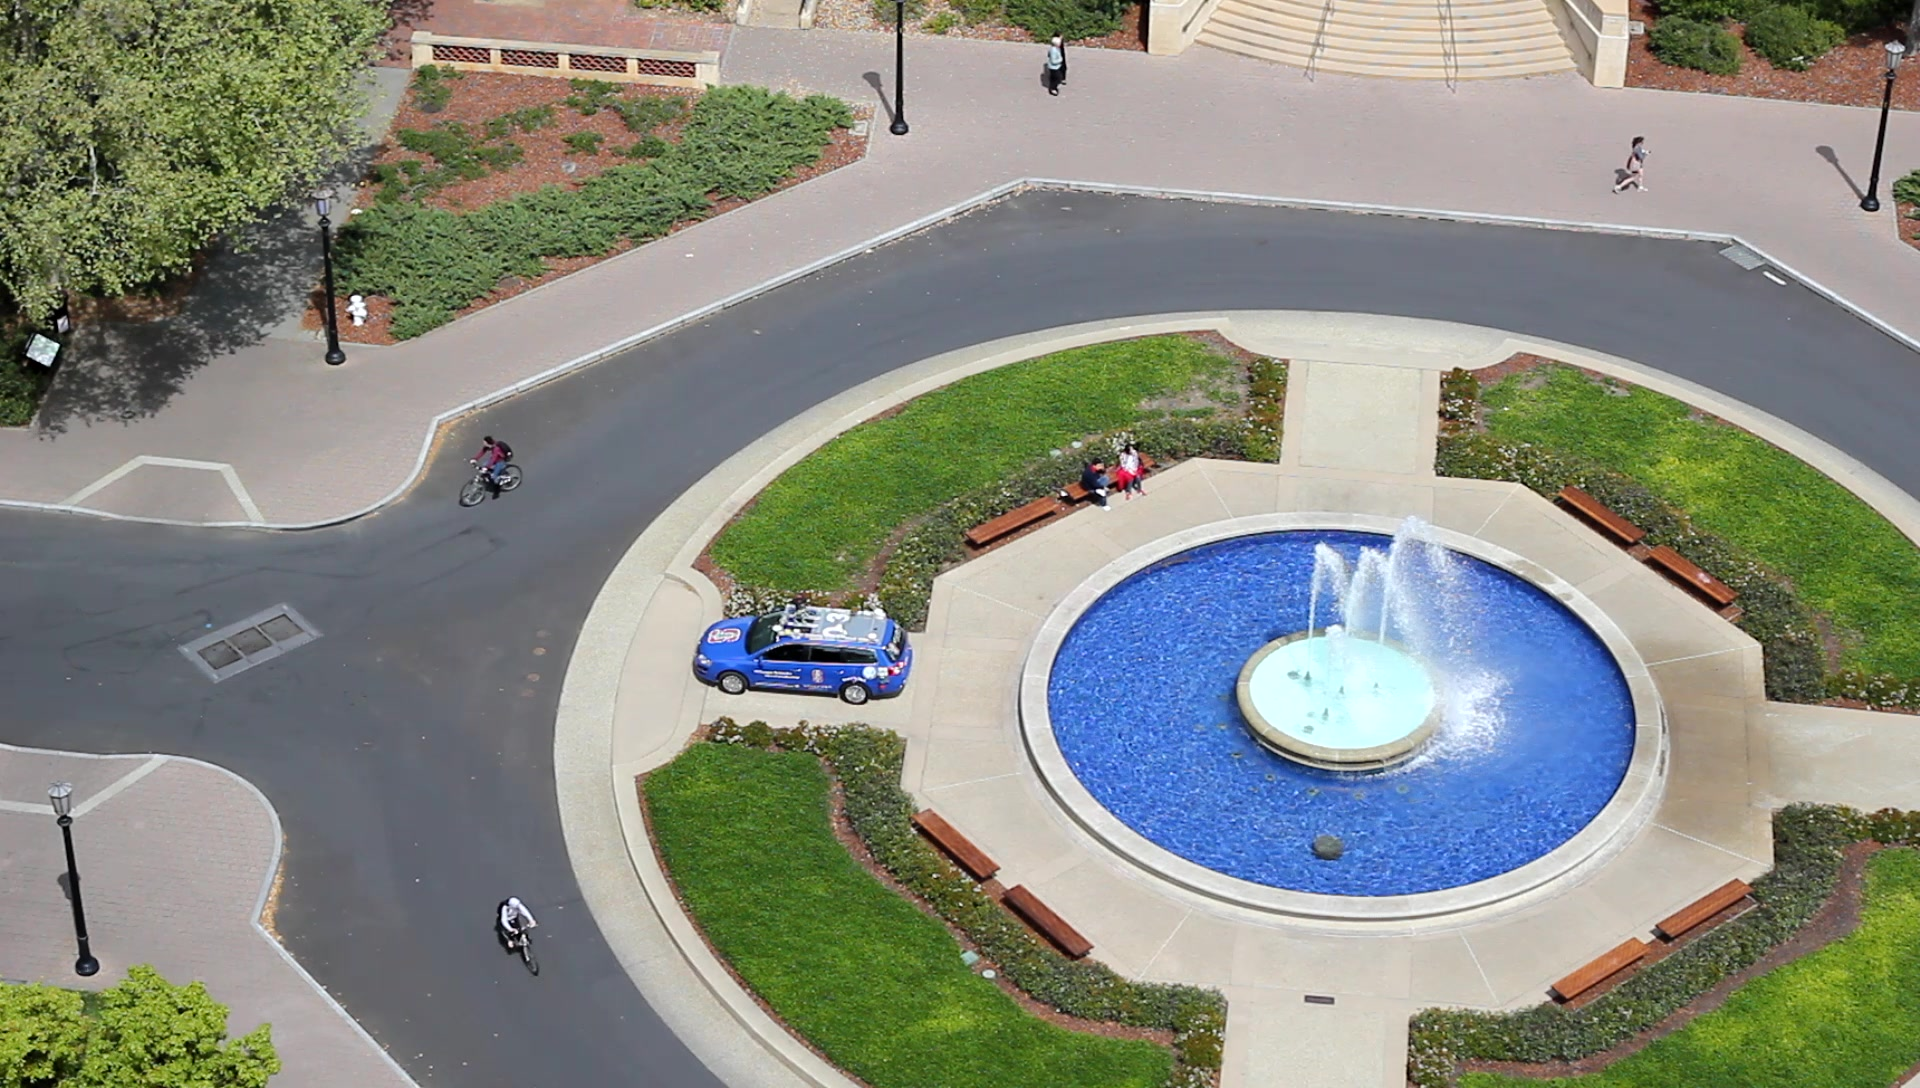
\epsfig{file=figs/campus_000042.eps, angle=0, width=1\linewidth, clip=}
%\caption{\label{fig:campus_000042} a) Input image frame.}
%\end{minipage}
%\addtocounter{figure}{-1}
%\begin{minipage}[b]{0.37\linewidth}
%\centering
%\epsfig{file=figs/RoIs_campus_000042.eps, angle=0, width=1\linewidth, clip=}
%\caption{\label{fig:campus_000042} b) Regions of Interest generated by Saliency Model.}
%\raggedright
%\epsfig{file=figs/RoIs_campus_000042.eps, angle=0, width=1\linewidth, clip=}
%\caption{\label{fig:campus_000042} c) Objects classified by HMAX Model.}
%\end{minipage}
%\end{figure*}
